\documentclass[a4paper,10pt]{book}

\usepackage{color}
\usepackage{bm}
\usepackage{amsmath}
\usepackage{appendix}
\usepackage{xspace}
\usepackage{a4wide}
\usepackage{wrapfig}
\usepackage[numbers,comma,sort&compress]{natbib}
\usepackage{graphicx}
%\usepackage{xstring}
\usepackage{listings,xcolor,courier}
%\usepackage{draftcopy}
\usepackage{longtable}
\usepackage{paralist}
%\usepackage{fancyvrb}
\usepackage{listings}

\usepackage
[dvips, %or dvips or pdftex
pagebackref, %or backref
colorlinks=true,
linkcolor=webgreen, %defined below
filecolor=webbrown, %defined below
citecolor=webgreen, %defined below
pdftitle={VOTCA-CT manual},
pdfauthor={},
pdfsubject={VOTCA-CT},
pdfkeywords={charge transport organic semiconductors},
bookmarksopen=false,
pdfpagemode=UseNone]{hyperref}

\definecolor{webgreen}{rgb}{0,.5,0}
\definecolor{webbrown}{rgb}{.6,0,0}
\pdfcompresslevel=9

\usepackage[T1]{fontenc}
%\usepackage{times}
\usepackage{type1cm}

\def\bibsection{%
    \section*{References}%
}

\begin{document}

\input{hgid}

\newcommand{\equ}[1]{eq.~\eqref{equ:#1}}
\newcommand{\Equ}[1]{Eq.~\eqref{equ:#1}}
\newcommand{\fig}[1]{figure~\ref{fig:#1}}
\newcommand{\Fig}[1]{Figure~\ref{fig:#1}}
\newcommand{\sect}[1]{section~\ref{sec:#1}}

\newcommand{\slink}[2]{\hyperref[#1]{#2}}


\newcommand{\xml}{XML\xspace}
\newcommand{\gromacs}{GROMACS\xspace}
\newcommand{\gaussian}{GAUSSIAN\xspace}
\newcommand{\turbomole}{TURBOMOLE\xspace}
\newcommand{\tinker}{TINKER\xspace}
\newcommand{\dipro}{DIPRO\xspace}

\newcommand{\Alq}{$\mathrm{Alq}_3$\xspace}
\newcommand{\dcvt}{DCV2T\xspace}

\newcommand{\xyz}{\texttt{geometry.xyz}\xspace}
\newcommand{\orb}{\texttt{zindo.orb}\xspace}
\newcommand{\votcactp}{{\MakeUppercase{votca-ctp}}\xspace}

\newcommand{\calculator}{\hyperref[sec:calculators]{calculator}\xspace}

\newcommand{\xmloptions}{\texttt{options.xml}\xspace}
\newcommand{\xmlcsg}{\hyperref[sec:xmlmap]{\texttt{map.xml}}\xspace}
\newcommand{\xmlsegments}{\hyperref[sec:xmlsegments]{\texttt{segments.xml}}\xspace}
\newcommand{\sqlstate}{\hyperref[sec:statefile]{\texttt{state.db}}\xspace}
\newcommand{\topology}{\texttt{topol.tpr}\xspace}
\newcommand{\trajectory}{\texttt{traj.xtc}\xspace}

\newcommand{\opt}{\texttt{{ -}o}\xspace}
\newcommand{\seg}{\texttt{{ -}s}\xspace}
\newcommand{\sql}{\texttt{{ -}f}\xspace}
\newcommand{\exe}{\texttt{{ -}e}\xspace}
\newcommand{\tpl}{\texttt{{ -}t}\xspace}
\newcommand{\csg}{\texttt{{ -}m}\xspace}
\newcommand{\trj}{\texttt{{ -}c}\xspace}


\newcommand{\refcalc}{\hyperref[ref:calculators]{calculators}\xspace}

\newcommand{\overlap}{\hyperref[prog:moo_overlap]{\texttt{moo\_overlap}}\xspace}
\newcommand{\ctprun}{\hyperref[prog:ctp_run]{\texttt{ctp\_run}}\xspace}
\newcommand{\ctpmap}{\hyperref[prog:ctp_map]{\texttt{ctp\_map}}\xspace}
\newcommand{\ctpdipro}{\hyperref[prog:ctp_dipro]{\texttt{ctp\_dipro}}\xspace}

\newcommand{\sqlite}{\texttt{sqlite3}\xspace}
\newcommand{\sqlconjsegproperties}{\texttt{conjseg\_properties}\xspace}
\newcommand{\sqlconjsegs}{\texttt{conjsegs}\xspace}
\newcommand{\sqlmolecules}{\texttt{molecules}\xspace}
\newcommand{\sqlpairintegrals}{\texttt{pairintegrals}\xspace}
\newcommand{\sqlpairproperties}{\texttt{pairproperties}\xspace}
\newcommand{\sqlpairs}{\texttt{pairs}\xspace}
\newcommand{\sqlrigidfragproperties}{\texttt{rigidfrag\_properties}\xspace}
\newcommand{\sqlrigidfrags}{\texttt{rigidfrags}\xspace}
\newcommand{\sqlframes}{\texttt{frames}\xspace}


\newcommand{\suggestion}[1]{{\color{red}SUGGESTION: #1}}

\newcommand{\segmentref}[1]{segments.#1}
\newcommand{\segmentopt}[1]{\hyperlink{\segmentref{#1}}{\StrSubstitute{#1}{_}{\_}}\xspace}
\newcommand{\calcref}[1]{#1}
\newcommand{\calcopt}[1]{\hyperlink{\calcref{#1}}{\StrSubstitute{#1}{_}{\_}}\xspace}

\newcommand{\calc}[1]{\hyperref[calc:#1]{\texttt{#1}}\xspace}

\def\bibsection{%
    \chapter*{Bibliography}%
    \addcontentsline{toc}{chapter}{Bibliography}
}

\renewcommand*{\showkeyslabelformat}[1]{{\normalfont\tiny\sffamily#1}}
\definecolor{refkey}{rgb}{1,0,0}
\definecolor{labelkey}{rgb}{1,0,0}


\frontmatter
\begin{titlepage}

\center{\fontsize{4cm}{5cm}\selectfont VOTCA}
\center{\fontsize{1.5cm}{3cm}\selectfont USER MANUAL}

\vspace*{3cm}
\center{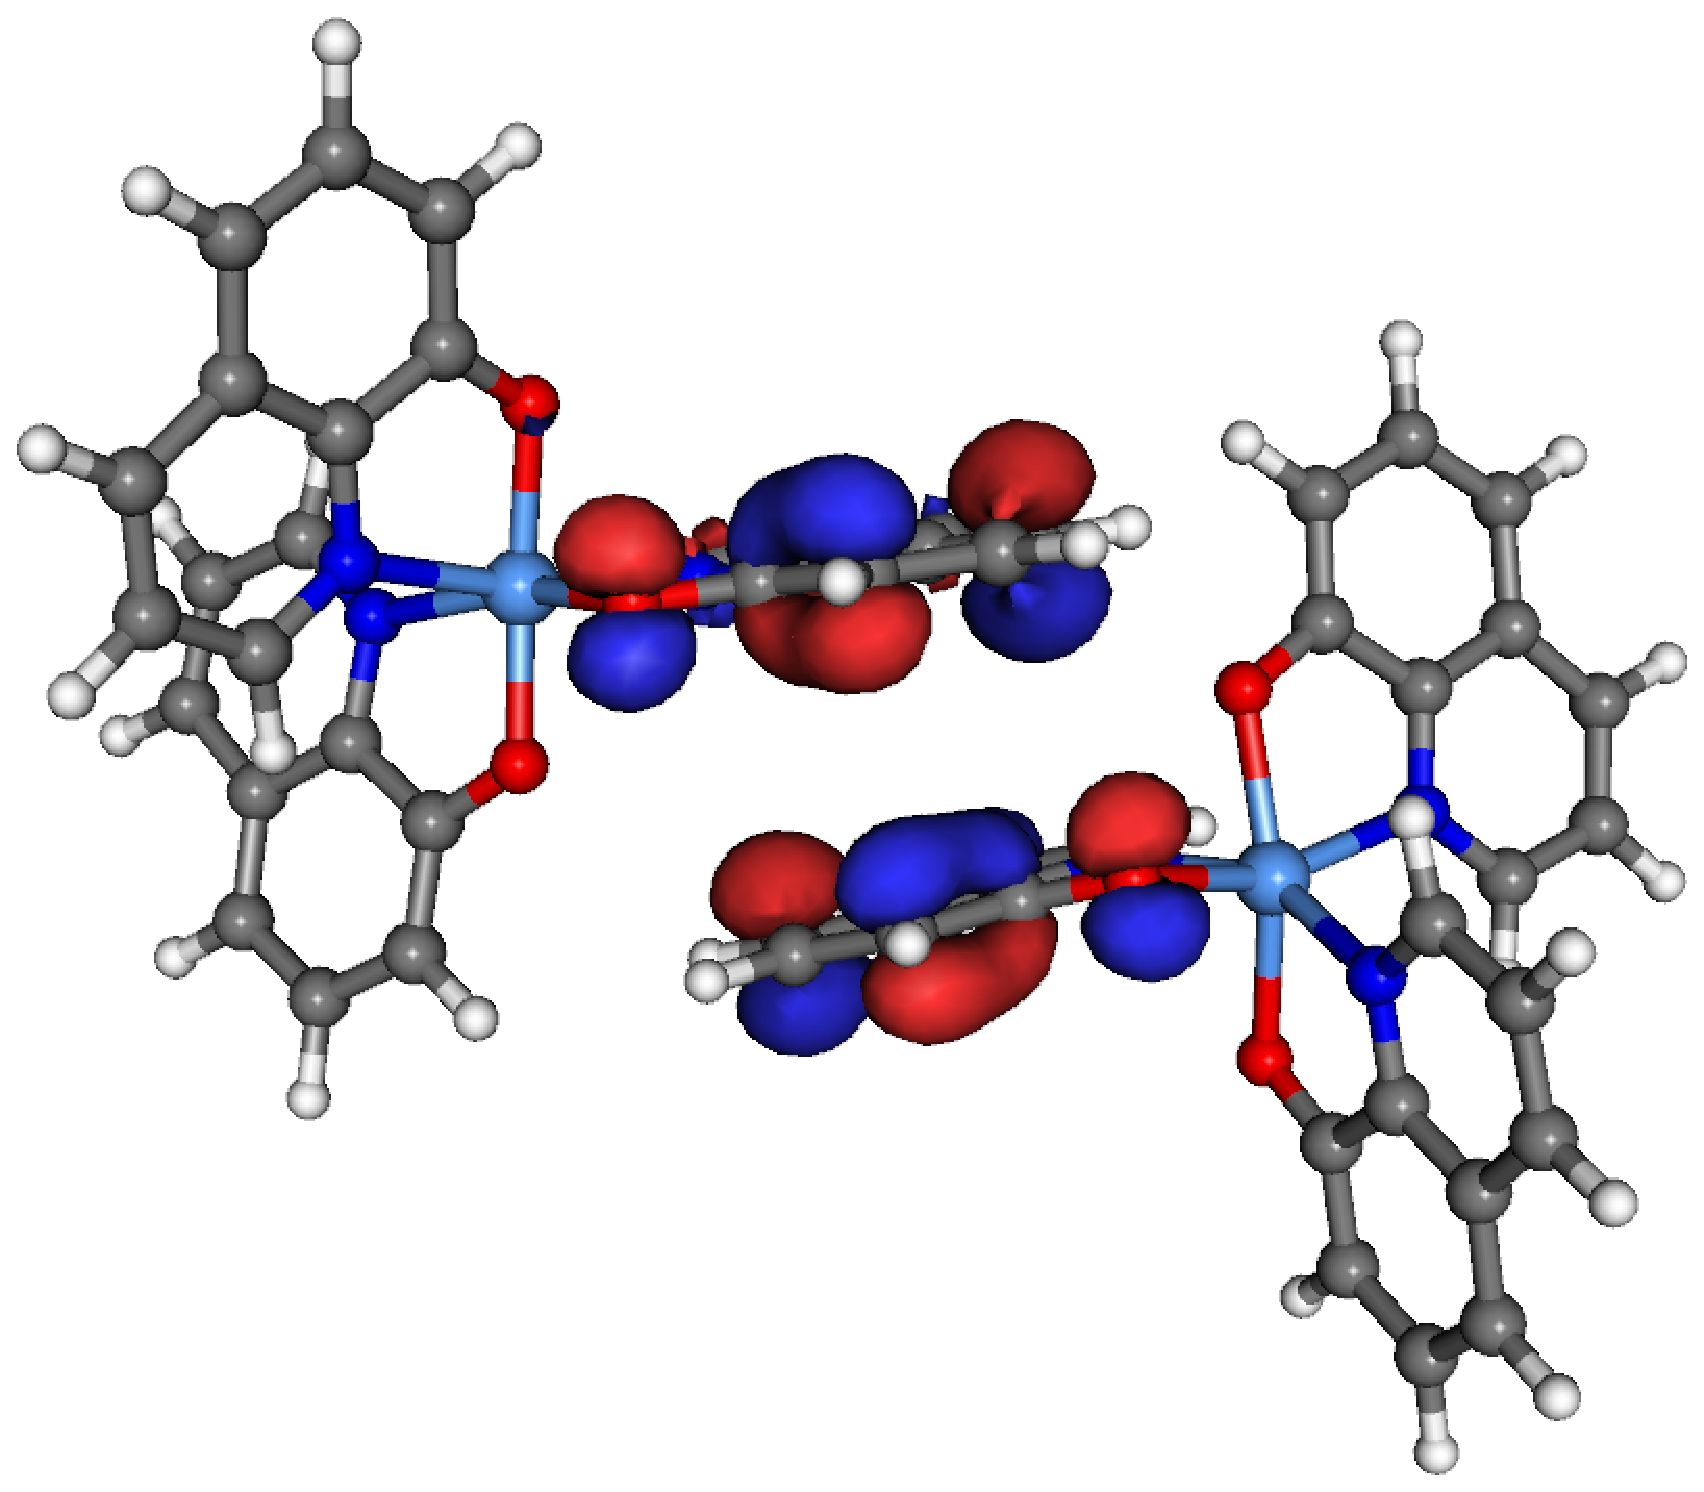
\includegraphics[width=\columnwidth]{fig/logo}}
\vspace*{1cm}
\vfill
\vspace*{1.4cm}
\center{\large{\today}}
\vspace*{-0.3cm}
\center{\footnotesize{Version: \gitid}}
\center{\footnotesize{Programs version: \csgid}}

\vspace*{1cm}
%\center{
\large{\copyright \hspace*{0.1cm} VOTCA development team}
%}
\vspace*{0.5cm}

\htmladdnormallink{\color{black}\large{www.votca.org}}{http://www.votca.org}
\end{titlepage}

\section*{Disclamer}
This manual is not complete. The best way to start using the software is to look at provided tutorials. The reference section is generated automatically from the source code, so please make sure that your software and manual versions match.  

\section*{Citations}
Development of this software depends on academic research grants. If you are using the package, please cite the  following papers \\

\vspace{0.1cm}
\noindent
\cite{mashayakrelative} Relative entropy and optimization-driven coarse-graining methods in VOTCA, \\
S.Y. Mashayak, Mara Jochum, Konstantin Koschke, N.R. Aluru, Victor R\"uhle, and Christoph Junghans,\\
\htmladdnormallink{  {\itshape Plos One} (2015)}
{http://dx.doi.org/10.1371/journal.pone.0131754}

\vspace{0.1cm}
\noindent
\cite{ruhle2011hybrid} Hybrid approaches to coarse-graining using the VOTCA package: liquid hexane, \\
Victor R\"uhle and Christoph Junghans, \\
\htmladdnormallink{  {\itshape Macromol. Theory Simul.} 20, 472 (2011)}
{http://dx.doi.org/10.1002/mats.201100011}

\vspace{0.1cm}
\noindent
\cite{Ruehle:2009.a} Versatile Object-oriented Toolkit for Coarse-graining Applications \\
Victor R\"uhle, Christoph Junghans, Alexander Lukyanov, Kurt Kremer, and Denis Andrienko \\
\htmladdnormallink{  {\itshape J. Chem. Theor. Comp.} 5, 3211, 2009}
{http://dx.doi.org/10.1021/ct900369w}

\section*{Development}
The core development is currently taking place at the Los Alamos National Laboratory and Max Planck Institute for Polymer Research, Mainz, Germany.

\section*{Copyright}
\votca is free software. The entire package is available under the Apache License. For details, check
the LICENSE file in the source code. The \votca source code is available on our homepage, \htmladdnormallink{\color{black}www.votca.org}{http://www.votca.org}.

\vfill

\thispagestyle{empty}
\cleardoublepage

\tableofcontents
\cleardoublepage
\mainmatter
\chapter{Introduction}
\label{sec:introduction}

Charge carrier dynamics in an organic semiconductor can often be described in terms of charge hopping between localized states. The hopping rates depend on electronic coupling elements, reorganization energies, and driving forces, which vary as a function of position and orientation of the molecules.  The exact evaluation of these contributions in a molecular assembly is computationally prohibitive. Various, often semi-empirical, approximations are employed instead. The purpose of \votcactp is to simplify the workflow for charge transport simulations, provide a uniform error-control for the methods, flexible platform for their development, and eventually allow in silico pre-screening of organic semiconductors for specific applications. 

The toolkit is implemented using modular concepts introduced earlier in the Versatile Object-oriented Toolkit for Coarse-graining Applications (VOTCA)~\cite{ruehle_versatile_2009}. The VOTCA structures are adapted to reading atomistic trajectories, mapping them onto conjugated segments and rigid fragments, and substituting (if needed) rigid fragments with the optimized copies. 

The \hyperref[sec:moo]{molecular orbital overlap} module calculates electronic coupling elements between  conjugated segments from the corresponding molecular orbitals. It relies on the semi-empirical INDO Hamiltonian and molecular orbitals in the format provided by the \gaussian package. An alternative,  \hyperref[sec:dft]{density-functional based approach}, has interfaces to the \gaussian and \turbomole packages. An interface to the \tinker package is provided for calculations of electrostatic and polarization contributions to energetic disorder. 

The  \hyperref[sec:kmc]{kinetic Monte Carlo module} reads in the neighbor list, site coordinates, and hopping rates and performs charge dynamics simulations using either periodic boundary conditions or charge sources and sinks. 

The toolkit is written as a combination of modular C++ code and scripts. The data transfer between programs is implemented via a state file or database, which is also used to restart simulations. Analysis functions and most of the calculation routines are encapsulated by using the observer pattern~\cite{gamma_design_1995} which allows the implementation of new functions as individual modules.
\chapter{Theoretical background}
\label{sec:theory}

\section{Workflow}
A typical workflow of charge transport simulations is depicted in \fig{workflow}. The first step is the simulation of an \hyperref[sec:morphology]{atomistic morphology}, which is then partitioned on \hyperref[sec:mapping]{hopping sites}. The coordinates of the hopping sites are used to construct a list of pairs of molecules (neighbor list). 

\begin{figure}[h]
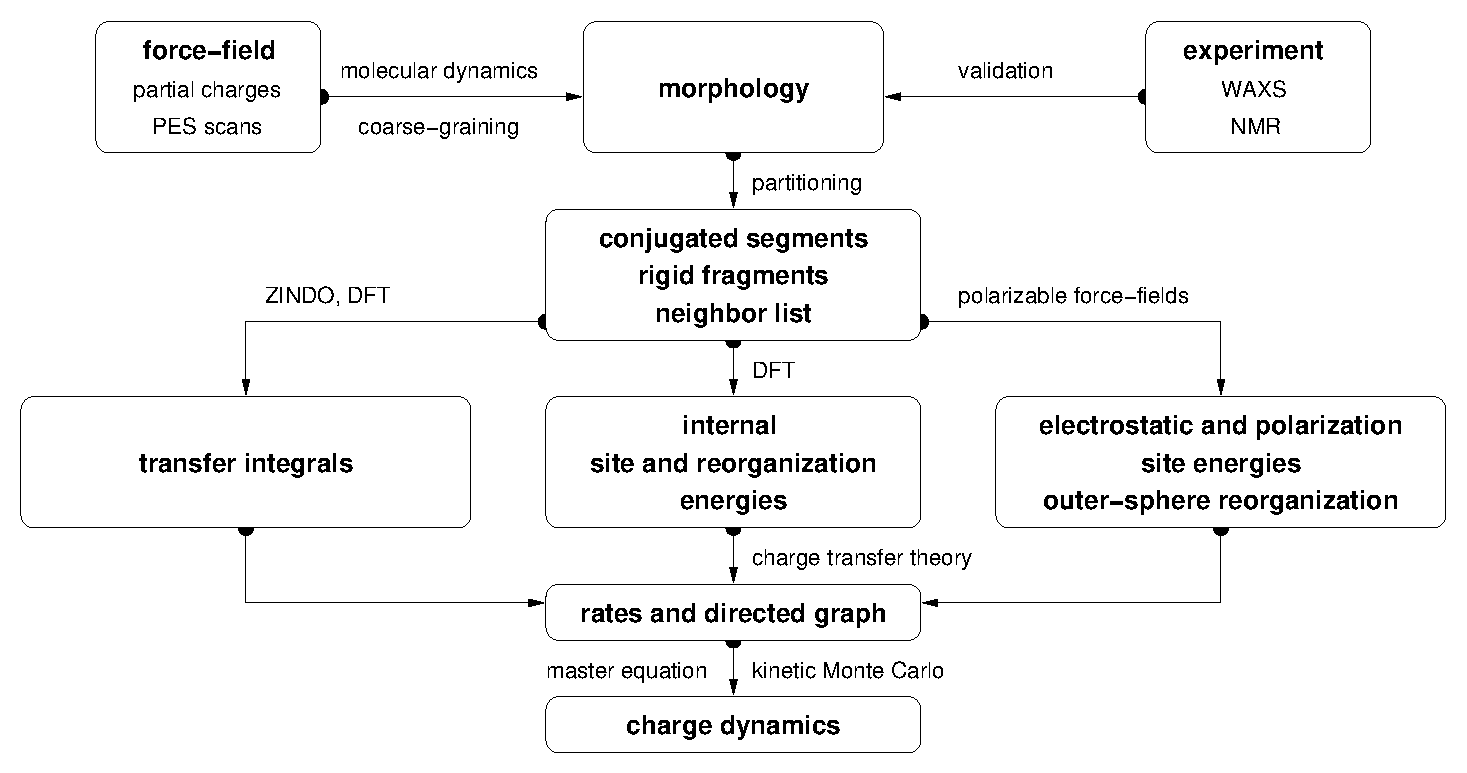
\includegraphics[width=\textwidth]{fig/workflow/workflow}
 \caption{%
   Workflow for microscopic simulations of charge transport.  %
   \label{fig:workflow}}
\end{figure}

For each pair an \hyperref[sec:transfer_integrals]{electronic coupling element}, a reorganization energy, a driving force, and eventually the hopping rate are evaluated. The neighbor list and hopping rates define a directed graph. The corresponding master equation is solved using the  \hyperref[sec:kmc]{kinetic Monte Carlo method}, which allows to explicitly monitor the charge dynamics in the system as well as to calculate time- or ensemble averages of occupation probabilities, charge fluxes, correlation functions, and field-dependent mobilities.


\section{Conjugated segments and rigid fragments}
\label{sec:conjugated_segments}

With the morphology at hand, the next step is partitioning the system on hopping sites, or conjugated segments, and calculating charge transfer rates between them. Physically intuitive arguments can be used for the partitioning,  which reflects the localization of the wave function of a charge. For most organic semiconductors, the molecular architecture includes relatively rigid, planar $\pi$-conjugated systems, which we will refer to as rigid fragments. A conjugated segment can contain one or more of such rigid fragments, which are linked by bonded degrees of freedom. The dynamics of these degrees of freedom evolves on timescales much slower than the frequency of the internal promoting mode. In some cases, e.g. glasses, it can be `frozen' due to non-bonded interactions with the surrounding molecules.

\begin{wrapfigure}{ht}{0.5\linewidth}
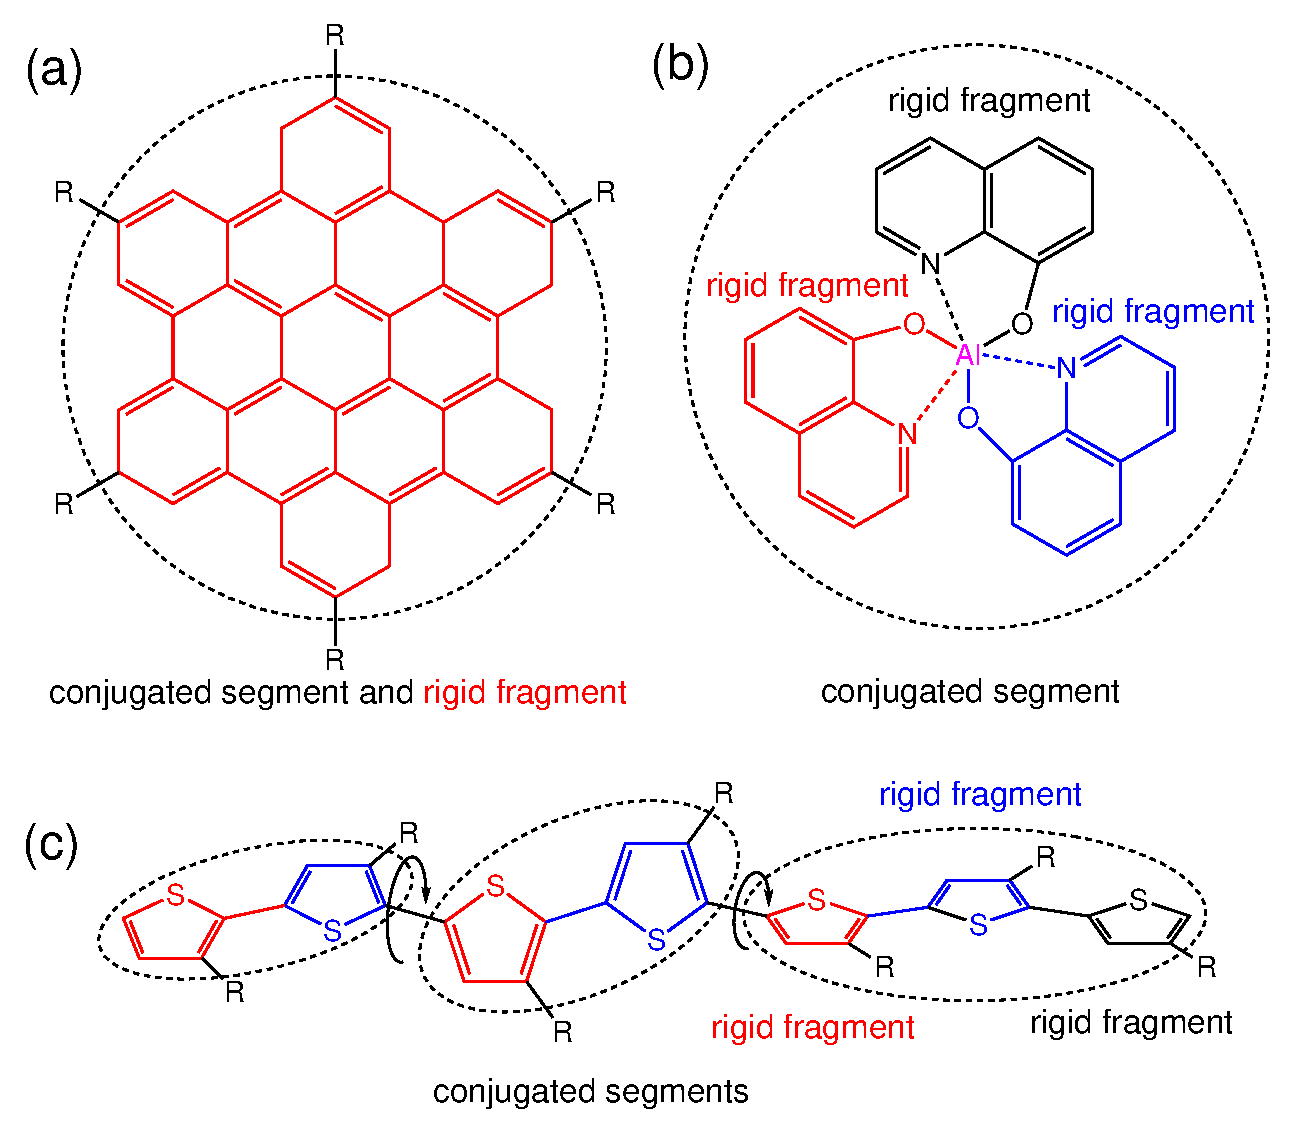
\includegraphics[width=\linewidth]{fig/conjugated_segment/fragment_segment}
\caption{\small The concept of conjugated segments and rigid fragments. Dashed lines indicate conjugated segments while colors denote rigid fragments. (a) Hexabenzocoronene: the $\pi$-conjugated system is both a rigid fragment and a conjugated segment. (b) \Alq: the Al atom and each ligand are rigid fragments while the whole molecule is a conjugated segment. (c) Polythiophene: each repeat unit is a rigid fragment. A conjugated segment consists of one or more rigid fragments. One molecule can have several conjugated segments.}
\label{fig:segment}
\end{wrapfigure}


To illustrate the concept of conjugated segments and rigid fragments, three representative molecular architectures are shown in \fig{segment}. The first one is a typical discotic liquid crystal, hexabenzocoronene. It consists of a conjugated core to which side chains are attached to aid self-assembly and solution processing. In this case the orbitals localized on side chains do not participate in charge transport and the conjugated $\pi$-system is both, a rigid fragment and a conjugated segment. 
%
In \Alq, a metal-coordinated compound, a charge carrier is delocalized over all three ligands. Hence, the whole molecule is one conjugated segment. Individual ligands are relatively rigid, while energies of the order of $k_\text{B}T$ are sufficient to reorient them with respect to each other. Thus the Al atom and the three ligands are rigid fragments.
%
In the case of a conjugated polymer, one molecule can consist of several conjugated segments, while each backbone repeat unit is a rigid fragment. Since the conjugation along the backbone can be broken due to large out-of-plane twists between two repeat units, an empirical criterion, based on the dihedral angle, can be used to partition the backbone on conjugated segments~\cite{ruehle_multiscale_2010}. However, such intuitive partitioning is, to some extent, arbitrary and shall be validated by other methods~\cite{vukmirovi_charge_2008,vukmirovi_charge_2009,mcmahon_ad_2009}. 

After partitioning, an additional step is often required to remove bond length fluctuations introduced by molecular dynamics simulations, since they are already integrated out in the derivation of the rate expression. This is achieved by substituting respective molecular fragments with  rigid, planar $\pi$-systems optimized using first-principles methods. Centers of mass and gyration tensors are used to align rigid fragments, though a custom definition of local axes is also possible. Such a procedure also minimizes discrepancies between the force-field and first-principles-based ground state geometries of conjugated segments, which might be important for calculations of electronic couplings, reorganization energies, and intramolecular driving forces. 

Finally, a list of neighboring conjugated segments is constructed. Two segments are added to this list if the distance between centers of mass of {\em any} their rigid fragments is below a certain cutoff. This allows neighbors to be selected on a criterion of minimum distance of approach rather than center of mass distance, which is useful for molecules with anisotropic shapes.

\chapter{Input files}
\label{sec:mapping}

\xml-based input files specify atomistic topology, coarse-grained topology, and define conjugated segments. In addition, practically every \calculator requires options provided in a separate \xml file.

\section{Atomistic topology}
\label{sec:atomistic}
\subsection{\gromacs topology}
If you are using \gromacs for generating atomistic configurations, it is possible to directly use the topology file provided by \gromacs (\texttt{topology.tpr}). In this case the residue and atom names should match those used  in the coarse-grained topology and conjugated segment definitions. 

\subsection{Custom topology}
The custom topology can also be defined using an \xml file. Moreover, it s possible to partially overwrite the information provided in, for example, \gromacs topology file. We will illustrate how to create a custom topology file using \dcvt. The structure of \dcvt, together with atom type definitions, is shown in fig.~\ref{fig:dcv2t_at}. \dcvt has two thiophene (THI) and two dicyanovinyl (NIT) residues. The pdb file which contains residue types, residue numbering, atom names, atom types, and atom coordinates is shown in listing~\ref{list:pdb}.

\clearpage
\begin{figure}[ht]
\centering
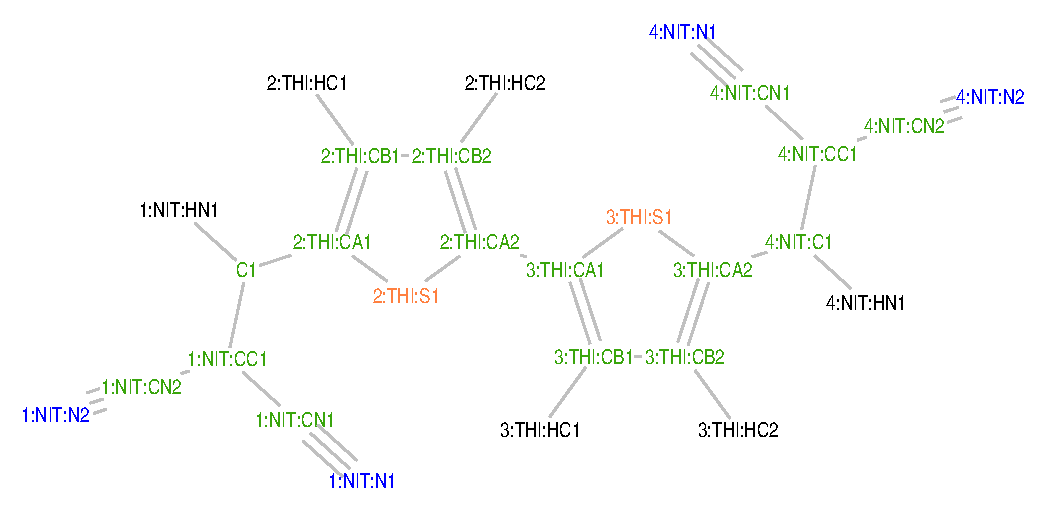
\includegraphics[width=0.8\textwidth]{./fig/chemical_structure/dcv2t_atom_types}
\caption{\small \dcvt with atoms labelled according to \texttt{residue\_number:residue\_name:atom\_name}. There are four residues and two residue types: thiophene (THI) and dicyanovinyl (NIT). The corresponding pdb file is shown in listing~\ref{list:pdb}.}
\label{fig:dcv2t_at}
\end{figure}

\lstinputlisting[
  language=XML,
  basicstyle=\ttfamily\small,
  stringstyle=\ttfamily\small,
  showstringspaces=false,
  frame=lines,
  label=list:pdb, 
  morekeywords={HETATM,THI,NIT},
  caption={\small pdb file of \dcvt.}]%
{./fig/chemical_structure/dcv2t.pdb}
\clearpage

\section{Mapping file}
\label{sec:xmlmap}
The mapping file (referred here as \xmlcsg) is used by the program \ctpmap to convert an atomistic trajectory to a trajectory with conjugated segments and rigid fragments. 
This trajectory is stored in a \slink{statefile}{state file} and contains positions, names, types of atoms belonging to rigid fragments. 
The description of the mapping options is given in table \ref{tab:map}. An example of \xmlcsg for a \dcvt molecule is shown in listing~\ref{list:map}. 
%
\begin{table}[h]
\label{tab:map}
\caption{Description of the \xml mapping file (\xmlcsg).}
\rowcolors{1}{invisiblegray}{white} {\footnotesize \input{reference/xml/map.xml}}
\end{table}
%
% Define new language for listings.
\lstdefinelanguage{MXML} {
   basicstyle=\ttfamily\scriptsize,
   sensitive=true,
   morecomment=[s][\color{gray}\rmfamily\itshape]{<!--}{-->}, 
   showstringspaces=false,
   numberstyle=\scriptsize,
   numberblanklines=true,
   showspaces=false,
   breaklines=true,
   showtabs=false,
   alsoletter={:},
   keywords = [1]
   { topology,molecules,molecule,name,mdname,segments,segment,fragments,fragment,mdatoms,qmatoms,localframe,weights},
   keywordstyle={[1]\color{blue}},
}

\lstinputlisting[
 language=MXML,
 label=list:map,
 caption={Examle of \xmlcsg for \dcvt. Each rigid fragment (coarse-grained bead) is defined by a list of atoms. Atom numbers, names, and residue names should correspond to those used in \gromacs topology (see the corresponing listing \ref{list:pdb} of the pdb file).}]%
{./input/dcv2t/map.xml}

\section{Conjugated segments}
\label{sec:xmlsegments}

The file describing hopping sites, or conjugated segments, is used by practically all programs and calculators. It links the coarse-grained trajectory (positions and orientations of rigid fragments) and quantum-mechanical descriptions of all conjugated segments. The description of this \xml file (\xmlsegments) is given in table \ref{tab:segments}. An example for \dcvt is shown in listing~\ref{list:segments}.

\begin{table}[h]
\caption{Description of conjugated segments (\xmlsegments).} 
\label{tab:segments}
\rowcolors{1}{invisiblegray}{white} {\small \input{reference/xml/segments.xml} }
\end{table}

\lstset{
  language=XML,
  frame=lines,
  basicstyle=\ttfamily\footnotesize,
  identifierstyle=\color{red},
  keywordstyle=\color{blue},
  showstringspaces=false,
  columns=fullflexible,
  commentstyle=\color{gray}\rmfamily\itshape,
  morekeywords={segments,segment,coordinates,orbitals,basisset,torbital,reorganization,qneutral,qcharged,energy,beadconj,molname,name,map,weights},
}

\lstinputlisting[
 label=list:segments, 
 caption={\small \xml file describing \slink{segments}{conjugated segments}. Note that the mapping and weights for each segment are separated by a colon. 
}]%
{./input/segments.xml}





\chapter{Transfer Integrals}

\section{Semi-empirical}

\section{Density-functional}
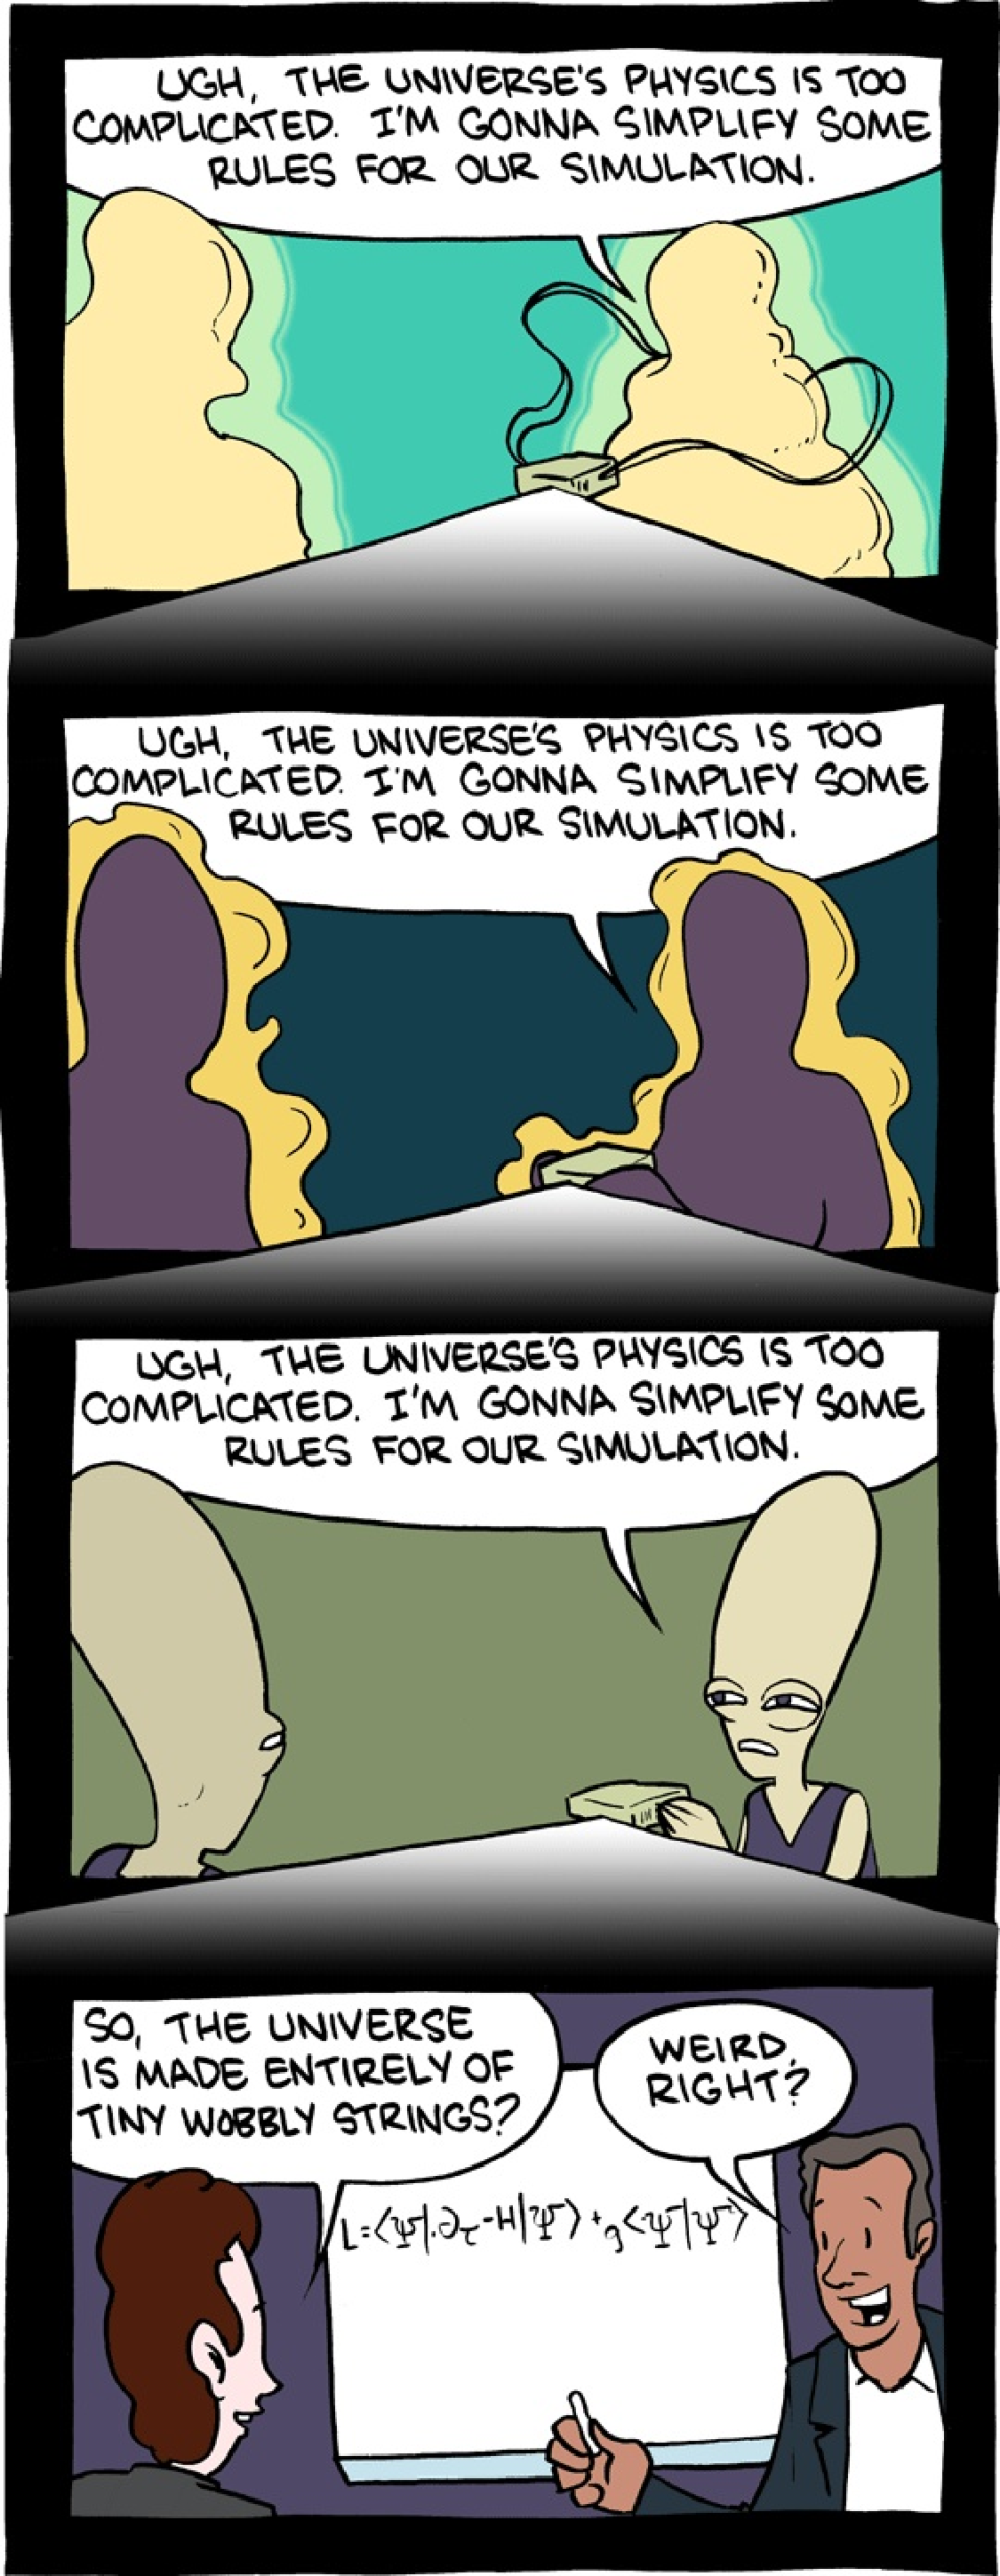
\includegraphics[width=0.4\linewidth]{fig/complicated}

\section{Site energies}
\label{sec:site_energies}
A charge transfer reaction between molecules $i$ and $j$ is driven by the site energy\index{site energy} difference, $\Delta E_{ij} = E_i - E_j$. Since the  transfer rate, $\omega_{ij}$, depends exponentially on $\Delta E_{ij}$ (see~\equ{marcus}) it is important to compute its distribution as accurately as possible.  The total site energy difference has contributions due to \slink{sec:ext_field}{externally applied electric field}, \slink{sec:ecoulomb}{electrostatic interactions}, polarization effects, and \slink{sec:internal_energy}{internal energy} differences. In what follows we discuss how to estimate these contributions by making use of first-principles calculations and polarizable force-fields.

\subsection{Externally applied electric field}
\label{sec:ext_field}
The contribution to the total site energy\index{site energy!external field} difference due to an external electric field $\vec{F}$ is given by $\Delta E_{ij}^\text{ext} = q {\vec{F} \cdot \vec{r}_{ij}}$, where $q=\pm e$ is the charge and $\vec{r}_{ij} = \vec{r}_i  - \vec{r}_j $ is a vector connecting molecules $i$ and $j$. For typical distances between small molecules, which are of the order  of $1\,\unit{nm}$, and moderate fields of $F<10^8\,\unit{V/m}$ this term is always smaller than $0.1\, \unit{eV}$.

\subsection{Electrostatic energy}
\label{sec:ecoulomb}
\index{site energy!electrostatic}

Variations of the local electric field can result in large electrostatic contributions to the energetic disorder. Using the atomic partial charges of charged and neutral molecules, $\Delta E_{ij}^\text{el}$ can be computed from the site energies~\cite{kirkpatrick_columnar_2008}
\begin{equation}
E_{i}^\text{el}  = \frac{1}{4 \pi \epsilon_0} \sum_{a_i} \sum_{\substack{b_k   \\ k\neq i }}
\frac{ \left( q^c_{a_i} - q^n_{a_i} \right) q^n_{b_k}}{ \epsilon_\text{s} r_{a_i b_k}} 
\, ,
\label{equ:estatic}
\end{equation}
where $r_{a_i b_k}=|\vec{r}_{a_i} - \vec{r}_{b_k}|$ is the distance between atoms $a_i$ and $b_k$,   $\epsilon_\text{s}$ is the static relative dielectric constant.
%
The first sum extends over all atoms of molecule $i$, for which the site energy is calculated. The second sum reflects interactions with all atoms of neutral molecules $k \ne i$. By using \equ{estatic}, one assumes that the influence of conformational changes on partial charges and changes of the molecular geometry upon charging are small. In order to minimize finite size effects, we do not use spherical cutoff but apply the nearest image convention, that is sum over all neutral molecules in the box after centering the box around the charged molecule. 

The influence of polarization effects on the Coulomb interactions can be taken into account by using a relative dielectric constant in \equ{estatic}. Bulk values of  $\epsilon_\text{s} = 2-5$ for typical organic semiconductors uniformly scale all site energies but are not capable of describing polarization effects on a microscopic level. 
The contribution to $E_i^\text{el}$ from the first coordination shell is then underestimated due to overscreening and, as a result, the site-energy differences become artificially small. Alternatively, one can introduce a phenomenological distance-dependent screening function $\epsilon(r_{a_i b_k})$ in~\equ{estatic}~\cite{nagata_atomistic_2008}
\begin{equation}
\epsilon(r)=\epsilon_{\text{s}} - (\epsilon_{\text{s}} - 1)
\left( 1 + sr + \frac{1}{2}s^2r^2 \right) 
\mathrm{e}^{ -sr}\,,
\label{equ:epss}
\end{equation}
where the parameter $s$ is the inverse screening length. For a monovalent ion in water, for example, $\epsilon_{\text{s}}=80$ and $s=3\,\textrm{nm}^{-1}$~\cite{daggett_molecular_1991}. This screening function ensures that neighboring atoms interact via an unscreened Coulomb potential ($\epsilon \sim 1$) while the electrostatic interaction between atoms at large separations is screened as in the bulk. 

Evaluation of the electrostatic contribution is provided by the \calc{emultipole} \calculator. Atomistic partial charges for charged an neutral molecule are taken from files specified in the \xmlcsg files. Note that, in order to speed up calculations for both methods, a cutoff radius (for the molecular centers of mass) can be given in  \xmloptions.

The electrostatic site energies are saved to the \sqlstate file:
\votcacommand{Electrostatic site energies}{\cmdemlt}

\subsection{Internal energy}
\label{sec:internal_energy}

The contribution to the site energy difference due to different internal energies\index{site energy!internal} (see \fig{parabolas}) can be written as
\begin{equation}
 \Delta E_{ij}^\text{int}=
\Delta U_i - \Delta U_j = \left( U_{i}^{cC}-U_{i}^{nN}\right) - \left( U_{j}^{cC}-U_{j}^{nN}\right) \, ,
\label{equ:conformational}
\end{equation}
where $U_{i}^{cC(nN)}$ is the total energy of molecule $i$ in the charged (neutral) state and geometry.  $\Delta U_{i}$ corresponds to the adiabatic ionization potential (or electron affinity) of molecule $i$, as shown in~\fig{parabolas}. For one-component systems and negligible conformational changes $ \Delta E_{ij}^\text{int}=0$, while it is significant for donor-acceptor systems. 

Internal energies determined using quantum-chemistry need to be specified in \xmlcsg. The values are written to the \sqlstate using the calculator \calc{einternal} (see also \slink{sec:eintramolecular}{intramolecular reorganization energy}):
\votcacommand{Internal energies}{\cmdeint}

\chapter{Solving the master equation}
\label{sec:me}

Having determined the list of conjugated segments (hopping sites) and charge transfer rates between them, the next task is to solve the master equation which describes the time evolution of the system
%
\begin{equation}
\label{equ:master}
\frac{\partial P_\alpha}{\partial t} = \sum_{\beta} P_\beta \Omega_{\beta \alpha} - 
\sum_{\beta} P_\alpha \Omega_{\alpha \beta},
\end{equation}
%
where $P_\alpha$ is the probability of the system to be in a state $\alpha$ at time $t$ and $\Omega_{\alpha \beta}$ is the transition rate from state $\alpha$ to state $\beta$. A state $\alpha$ is specified by a set of site occupations, $\left\{ \alpha_i \right\}$, where $\alpha_i = 1 (0)$ for an occupied (unoccupied) site $i$, and the matrix $\hat{\Omega}$ can be constructed from rates $\omega_{ij}$.

The solution of \equ{master} is be obtained by using kinetic Monte Carlo (KMC) methods. KMC explicitly simulates the dynamics of charge carriers by constructing a Markov chain in state space and can find both stationary and transient solutions of the master equation. The main advantage of KMC is that only states with a direct link to the current state need to be considered at each step. Since these can be constructed solely from current site occupations, extensions to multiple charge carriers (without the mean-field approximation), site-occupation dependent rates (needed for the explicit treatment of Coulomb interactions), and different types of interacting particles and processes, are straightforward. To optimize memory usage and efficiency, a combination of the variable step size method~\cite{bortz_new_1975} and the first reaction method is implemented.
\chapter{Manual pages}
%
% if you want to refer to any of the tags specified here use the following command
% \segmentopt{crgunit_type.ChargeUnitType.posname}
%
\section{Programs}
\label{ref:programs}
\input{reference/programs/all}

\section{Calculators}
\label{ref:calculators}
\label{sec:calculators}

Calculator is a piece of code which computes specific system properties, such as site energies, transfer integrals, etc. \ctprun is a wrapper program which executes all calculators. The generic syntax is 

  \ctprun \exe \texttt{"calc1, calc2, ..."} \opt \xmloptions
\vskip 0.2cm
%
File \xmloptions lists all options needed to run a specific calculator. The format of this file is explained in listing~\ref{list:calc}. A complete list of calculators is given in the \refcalc reference section.
%
\lstinputlisting[label=list:calc, 
 caption={\small A part of the \xmloptions file with options for the \texttt{calculator\_name\{1,2\}} \refcalc.
}]{./reference/calculators.xml}

\input{reference/calculators/all}
\vfill

\section{Options}
\label{ref:options}
%\setdefaultleftmargin{0.8em}{0.8em}{0.8em}{0.8em}{0.8em}{0.8em}

\subsection{Mapping file}
\rowcolors{1}{invisiblegray}{white}
{\small 
\input{reference/xml/map.xml}
}
\vfill

\subsection{Conjugated segments}
\rowcolors{1}{invisiblegray}{white}
{\small 
\input{reference/xml/segments.xml}
}
\vfill

\subsection{Calculator options}
\rowcolors{1}{invisiblegray}{white}
{\small 
\input{reference/xml/options.xml}
}
\vfill


\bibliographystyle{achemso}
\bibliography{literature_short}

\end{document} 
